\documentclass[12pt]{article}
\usepackage{amsgen,amsmath,amstext,amsbsy,amsopn,amssymb}
%\usepackage[dvips]{graphicx,color}
\usepackage{graphicx,color,bm}
\usepackage{epsfig}
\usepackage{enumerate}
\usepackage{float}
\usepackage{multicol}
\usepackage{longtable}
\usepackage{verbatim}
\usepackage{hyperref}
\usepackage[utf8]{inputenc}
\usepackage[english]{babel}
\usepackage{commath}
\usepackage{tikz}
\usepackage{wrapfig,lipsum,booktabs}
\usepackage{subcaption}
%\setlength{\oddsidemargin}{0.1 in} \setlength{\evensidemargin}{-0.1
%in} \setlength{\topmargin}{-0.6 in} \setlength{\textwidth}{6.5 in}
%\setlength{\textheight}{8.5 in} \setlength{\headsep}{0.75 in}
%\setlength{\parindent}{0 in} \setlength{\parskip}{0.1 in}

\textwidth 6.3in \textheight 8.8in \topmargin -0.5truein
\oddsidemargin .15truein
\parskip .1in
\renewcommand{\baselinestretch}{1.00}  % double spaced
\renewcommand{\thesection}{\Roman{section}} 
\renewcommand{\thesubsection}{\thesection.\Roman{subsection}}
\newcommand*{\addheight}[2][.5ex]{%
	\raisebox{0pt}[\dimexpr\height+(#1)\relax]{#2}%
}
\usepackage{caption}

\begin{document}
	
\title{%
	CSE 515 HW }

\author{ Alexander Van Roijen}

\maketitle	
	
\begin{section}{4.6}
	\subsection{a}
	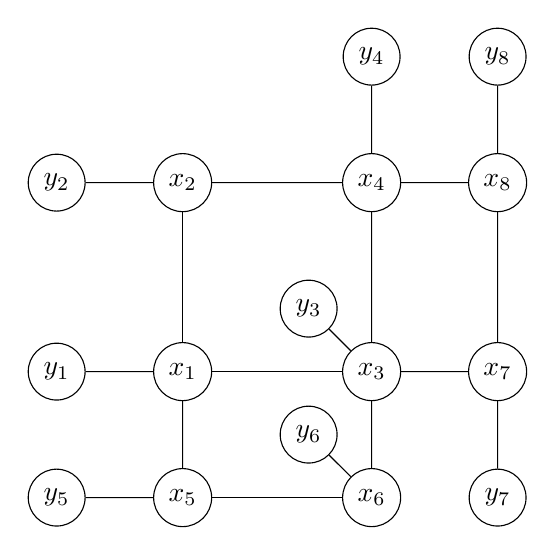
\begin{tikzpicture}
	[scale=.8,auto=left,every node/.style={circle,draw=black}]
	\node (n1) at (1,1) {$x_1$};
	\node (n2) at (1,4)  {$x_2$};
	\node (n3) at (4,1)  {$x_3$};
	\node (n4) at (4,4) {$x_4$};
	\node (n5) at (1,-1) {$x_5$};
	\node (n6) at (4,-1)  {$x_6$};
	\node (n7) at (6,1)  {$x_7$};
	\node (n8) at (6,4) {$x_8$};

	
	\node (y1) at (-1,1) {$y_1$};
	\node (y2) at (-1,4)  {$y_2$};
	\node (y3) at (3,2)  {$y_3$};
	\node (y4) at (4,6) {$y_4$};
	\node (y5) at (-1,-1) {$y_5$};
	\node (y6) at (3,0)  {$y_6$};
	\node (y7) at (6,-1)  {$y_7$};
	\node (y8) at (6,6) {$y_8$};	

	\foreach \from/\to in {n1/n2,n1/n3,n2/n4,n3/n4,n1/y1,n2/y2,n3/y3,n4/y4,n1/n5,n3/n6,n3/n7,n4/n8,n5/y5,n6/y6,n7/y7,n8/y8,n7/n8,n5/n6}
	\draw (\from) -- (\to);
	\end{tikzpicture}
	\\

	This represents one corner of our graph representing our image, so it would expand out much further, but this should suffice.
	\subsection{b}
	\begin{verbatim}
		For the background, we have
		mu = array([0.32488191, 0.3359058 , 0.15492575])	

		cov = [array([[0.07608524, 0.0709183 , 0.04026234],
		[0.0709183 , 0.06727482, 0.03855529],
		[0.04026234, 0.03855529, 0.02645081]]), 
		
		For the forground we have
		mu = array([0.70059092, 0.45043831, 0.04376236])
		
		cov = array([[0.05134831, 0.05985912, 0.00137747],
		[0.05985912, 0.08341228, 0.00235105],
		[0.00137747, 0.00235105, 0.00110494]])
	\end{verbatim}

	
	
	\subsection{c}
	\begin{figure}[H]
		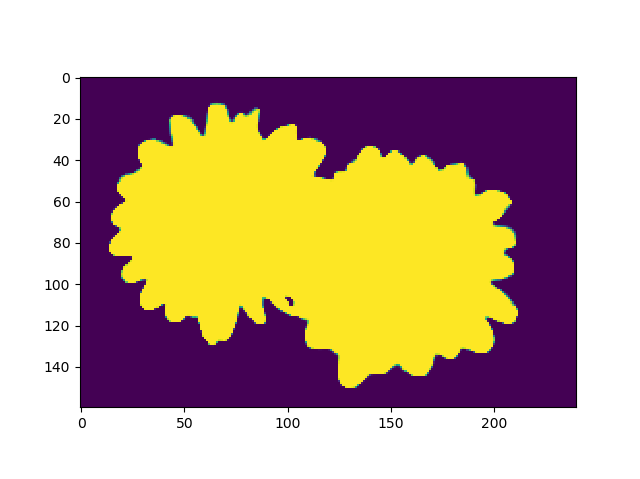
\includegraphics[width=0.7\textwidth]{30iterepi0_01.png}
		\caption{after 30 iterations of BP, $\epsilon = 0.01$}
	\end{figure}
	\subsection{c}
		\begin{figure}[H]
		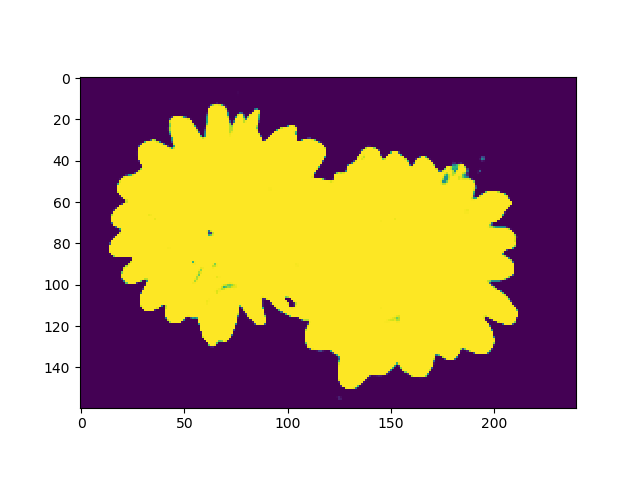
\includegraphics[width=0.7\textwidth]{iter1_0_01.png}
		\caption{after 1 BP iteration, $\epsilon = 0.01$}
	\end{figure}
	\begin{figure}[H]
		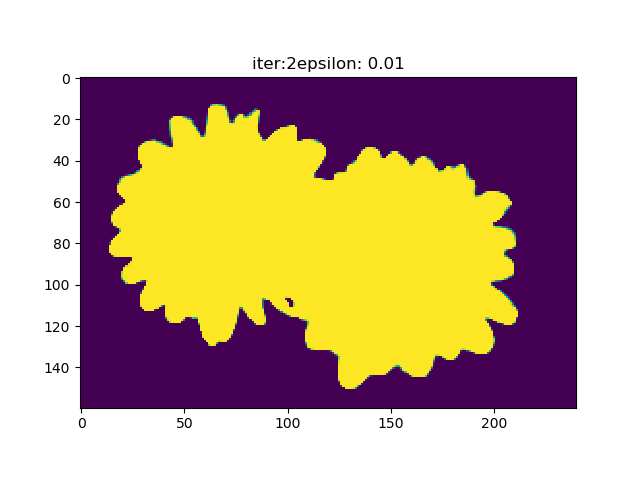
\includegraphics[width=0.7\textwidth]{iter2_0_01.png}
		\caption{after 2 BP iterations, $\epsilon = 0.01$}
	\end{figure}
		\begin{figure}[H]
		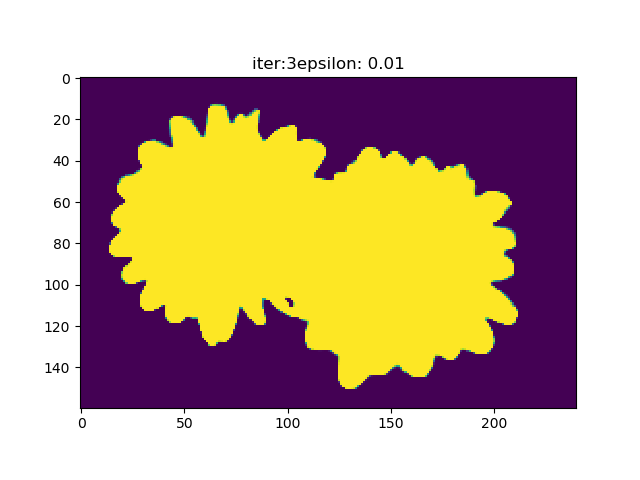
\includegraphics[width=0.7\textwidth]{iter3_0_01.png}
		\caption{after 3 BP iterations, $\epsilon = 0.01$}
	\end{figure}
		\begin{figure}[H]
		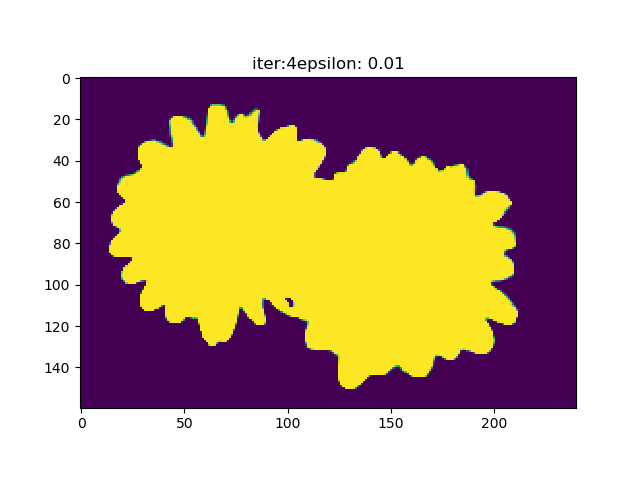
\includegraphics[width=0.7\textwidth]{iter4_0_01.png}
		\caption{after 4 BP iterations, $\epsilon = 0.01$}
	\end{figure}
As to be expected in a background foreground classification task, the greatest regions of uncertainty are around the edges of our flowers petals, as this is where nearby pixels are meant to be quite different from each other. 
\\
Overall, we see a great deal of change in labels and the confidence in them during the first and second iteration, but harder to tell in future iterations. Looking at figures below, we can see the edges are still being determined slightly during the next iterations between 2 and 3 and 3 and 4.
\begin{figure}[H]
	\centering
	\begin{subfigure}{.5\textwidth}
		\centering
		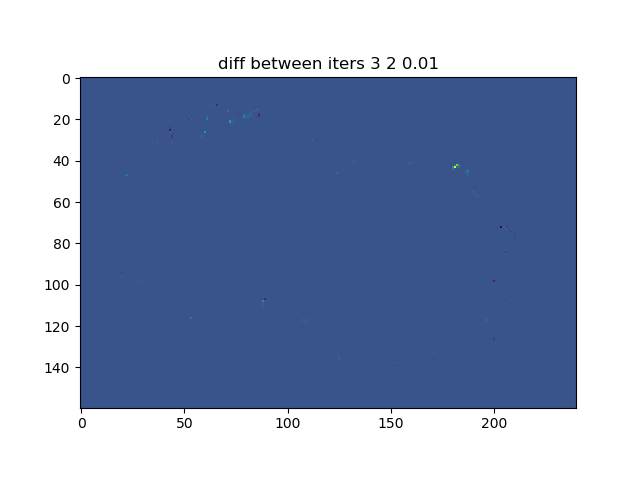
\includegraphics[width=.8\linewidth]{32diff.png}
		\label{23diff}
	\end{subfigure}%
	\begin{subfigure}{.5\textwidth}
		\centering
		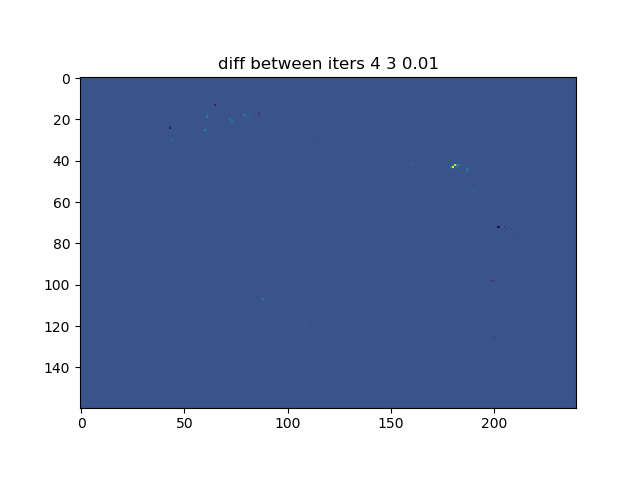
\includegraphics[width=.8\linewidth]{43diff.png}
		\label{34diff}
	\end{subfigure}
	\label{fig:test}
\end{figure}

Looking at these, we can see small regions of change around the upper right and left edges of our flowers. 
\\
\begin{figure}[H]
	\centering
	\begin{subfigure}{.5\textwidth}
		\centering
		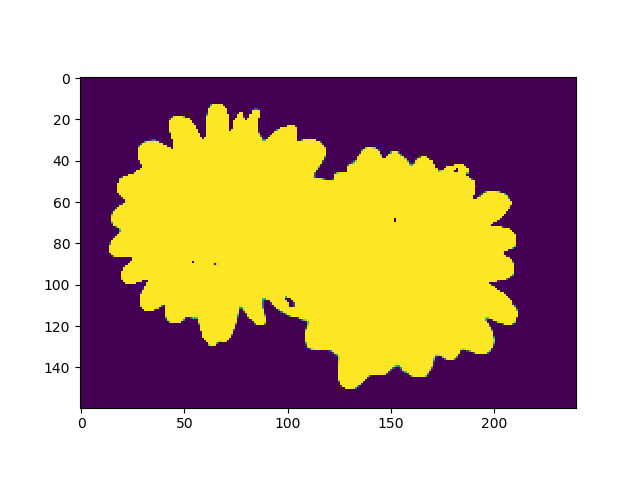
\includegraphics[width=.8\linewidth]{30iterepi0_00.png}
		\label{0epiresult30}
		\caption{30 iterations with $\epsilon = 0$}
	\end{subfigure}%
	\begin{subfigure}{.5\textwidth}
		\centering
		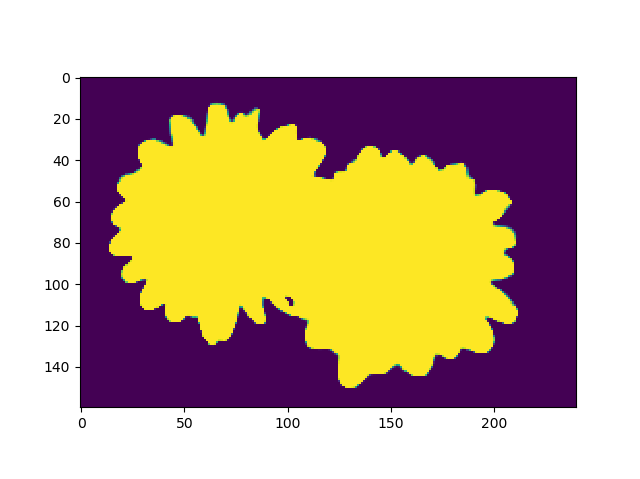
\includegraphics[width=.8\linewidth]{30iterepi0_01.png}
		\label{0epiresul1}
		\caption{30 iterations with $\epsilon = 0.01$}
	\end{subfigure}
	\label{fig:test2}
\end{figure}
The results are slightly similar, with a slight change in their edge cases, as to be expected. Overall, edges seem to be less sharply defined, a bit more rounded with a greater deal of uncertainty between background and foreground within different regions of hte flow

\begin{figure}[H]
	\centering
	\begin{subfigure}{.5\textwidth}
		\centering
		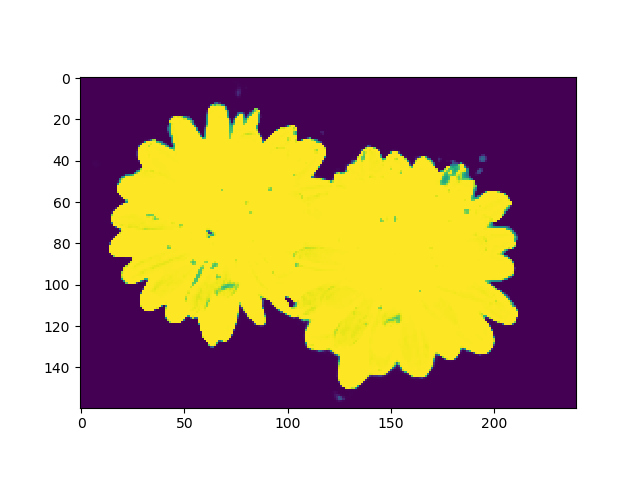
\includegraphics[width=.8\linewidth]{30iterepi0_01_46v2.png}
		\label{46res1}
		\caption{30 iterations with .6 and .4}
	\end{subfigure}%
	\begin{subfigure}{.5\textwidth}
		\centering
		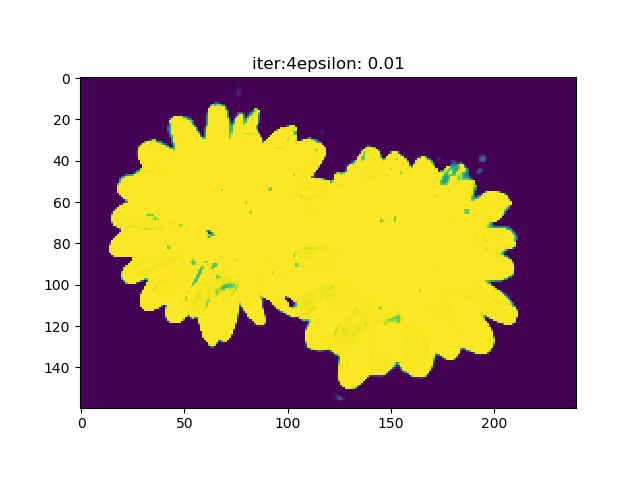
\includegraphics[width=.8\linewidth]{iter4_0_01_46v2.png}
		\label{46res2}
		\caption{4 iterations with .6 and .4}
	\end{subfigure}
	\label{fig:test3}
\end{figure}

\end{section}




\begin{section}{5.1}
	\subsection{a}
	$v_{i \rightarrow a}^{t+1}(x_i) = P(y_i|x_i)\Pi_{b\in \partial{i}-a}\tilde{v}_{b \rightarrow i}^t(x_i)$
	\\
	$\tilde{v}_{a \rightarrow i}^{t+1} (x_i) = \Sigma_{x_{\partial a-i}} \Pi_{j\in\partial a - i}v_{j \rightarrow a}^{t}(x_j)I(\bigotimes x_{\partial a}=1)$
	
	\subsection{b}
	For $v_{i \rightarrow a}^{t+1}(x_i)$ it will take $O(d_i)$ where $d_i$ is the number of factors that neighbor or connect to $i$ which is in general $O(l)$.
	\\
	\\
	For $\tilde{v}_{a \rightarrow i}^{t+1} (x_i)$ our time complexity is $O((|\partial a|-1)2^{|\partial a|-1}) = O(r2^{r})$. This is because we need to assure that our logic holds for every possible permutation of our nodes $I(\bigotimes x_{\partial a}=1)$. The additional $r$ comes from a need to multiply $r$ different messages together for each permutation.
	\\
	\\
	To reduce the complexity, we can expand our equation $\tilde{v}_{a \rightarrow i}^{t+1} (x_i)$ to get a general form of $v_{j \rightarrow a}^{t}(+1)*v_{h \rightarrow a}^{t}(+1) ... * v_{z \rightarrow a}^{t}(+1)I(\bigotimes x_{\partial a}=1) \\ + v_{j \rightarrow a}^{t}(-1)*v_{h \rightarrow a}^{t}(+1) ... * v_{z \rightarrow a}^{t}(+1)I(\bigotimes x_{\partial a}=1) \\ + v_{j \rightarrow a}^{t}(+1)*v_{h \rightarrow a}^{t}(-1) ... * v_{z \rightarrow a}^{t}(+1)I(\bigotimes x_{\partial a}=1) \\ + ... v_{j \rightarrow a}^{t}(-1)*v_{h \rightarrow a}^{t}(-1) ... * v_{z \rightarrow a}^{t}(-1)I(\bigotimes x_{\partial a}=1)$. Which then becomes a function of $x_i$ such that \\
	\\
	$\tilde{v}_{a \rightarrow i}^{t+1} (x_i = +1) = v_{j \rightarrow a}^{t}(+1)*v_{h \rightarrow a}^{t}(+1) ... * v_{z \rightarrow a}^{t}(+1)*1 \\ + v_{j \rightarrow a}^{t}(-1)*v_{h \rightarrow a}^{t}(+1) ... * v_{z \rightarrow a}^{t}(+1)*0 \\ + v_{j \rightarrow a}^{t}(+1)*v_{h \rightarrow a}^{t}(-1) ... * v_{z \rightarrow a}^{t}(+1)*0 \\ + ... v_{j \rightarrow a}^{t}(-1)*v_{h \rightarrow a}^{t}(-1) ... * v_{z \rightarrow a}^{t}(-1)*1$ (Note this last condition may be 0 or one depending on the carndinality of $r$).
	\\
	\\
	Similarly, the indicators would flip in 	$\tilde{v}_{a \rightarrow i}^{t+1} (x_i = -1)$. Thus, since both values end up with opposite signs, you would get the same results if you let each one cancel instead, meaning you add its negative counterpart $a+b + -b = a +0*b = a$. With this in mind, you can rewrite our equation into a product of \\
	\\
	$\tilde{v}_{a \rightarrow i}^{t+1} (x_i = +1) \propto (v_{j \rightarrow a}^{t}(+1)+v_{j \rightarrow a}^{t}(-1))\\ *(v_{h \rightarrow a}^{t}(+1)+v_{h \rightarrow a}^{t}(-1)) ... \\ * (v_{z \rightarrow a}^{t}(+1)+v_{z \rightarrow a}^{t}(-1)) \\
	+
	\\
	(v_{j \rightarrow a}^{t}(+1)-v_{j \rightarrow a}^{t}(-1))\\ *(v_{h \rightarrow a}^{t}(+1)-v_{h \rightarrow a}^{t}(-1)) ... \\ * (v_{z \rightarrow a}^{t}(+1)-v_{z \rightarrow a}^{t}(-1))
	$
	\\
	\\
	Taking the time to write this out, you can see you get some nice cancellations such as \\ \\
	$v_{j \rightarrow a}^{t}(-1)v_{h \rightarrow a}^{t}(+1)...v_{z \rightarrow a}^{t}(+1) - v_{j \rightarrow a}^{t}(-1)v_{h \rightarrow a}^{t}(+1)...v_{z \rightarrow a}^{t}(+1) = 0$ which satisfies exactly  $v_{j \rightarrow a}^{t}(-1)*v_{h \rightarrow a}^{t}(+1) ... * v_{z \rightarrow a}^{t}(+1)*0$. 
	\\
	\\
	Thus, we get $\tilde{v}_{a \rightarrow i}^{t+1} (x_i = +1) \propto  \Pi_{j\in\partial a - i}v_{j \rightarrow a}^{t}(+1)+v_{j \rightarrow a}^{t}(-1) + \Pi_{j\in\partial a - i}v_{j \rightarrow a}^{t}(+1)+v_{j \rightarrow a}^{t}(-1) $
	\\
	This satisfies our reduction in computation time to $O(d_a)$ as we only need to iterate over the neighbors values once
	\subsection{c}
	Initially, we have that $w^0=  P(W^0=-1) = P$(randomly chosen message from variable to factor is flipped) = $\epsilon$ as they are independent and we assume that $\forall x_i $ a message of 1 was sent.
	\\
	\\
	For subsequent time steps, with our messages as described, we get the probability of a message from a factor to a node taking value -1 only occurs when that factor received an odd number of -1 from the $r$ variable nodes it receives from. 
	\\
	\\
	So we can think of $z^t=P(Z^t=-1)$ as a binomial distribution with the parameters  $r$,$p= (w^{t})$. And we want the sum of all instance where the number of successes is odd.
	$z^t=P(Z^t=-1) = \Sigma_{i=1,3,..r} p^i(1-p)^{n-i}$. However, this can be reduced, as the number of odd values for a Binomial distribution $r$,$p$ gives$\frac{1-(1-2p)^{r-1}}{2}$
	\\
	\\
	Similarly,
	$w^{t+1} = P(W^{t+1}=-1) = (z^t)^{l-1} + \epsilon(1- (z^t)^{l-1} - (1-z^t)^{l-1})$ as all incoming messages from our factor must be -1 in order for it to be -1.
	\subsection{d}
	$w^{t+1} = ( \frac{1-(1-2p)^{r-1}}{2})^{l-1} + (1-\frac{1-(1-2p)^{r-1}}{2}^{l-1} - (1-\frac{1-(1-2p)^{r-1}}{2})^{l-1})\epsilon $ where $p = w^{t}$
	\\
	\\
	
	\begin{figure}[H]
		\centering
		\begin{subfigure}{.5\textwidth}
			\centering
			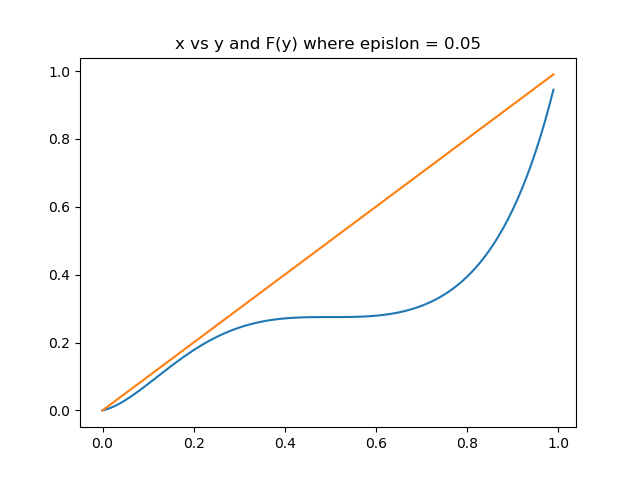
\includegraphics[width=.8\linewidth]{epi0_05q51.png}
			\label{51d1}
			\caption{$F(y)$ over various values from 0 to 1 with $\epsilon = 0.05$}
		\end{subfigure}%
		\begin{subfigure}{.5\textwidth}
			\centering
			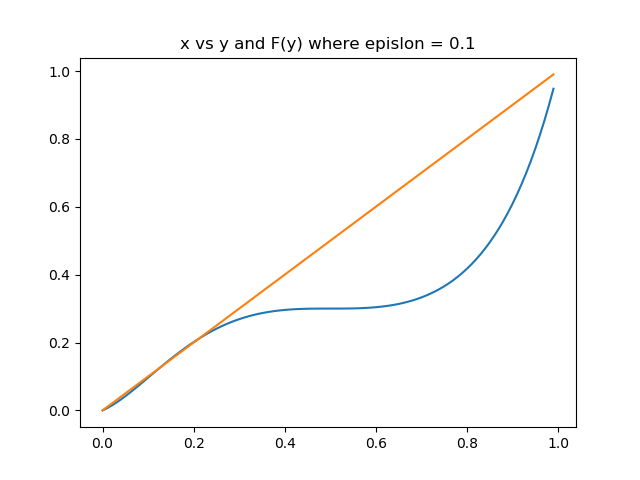
\includegraphics[width=.8\linewidth]{epi0_1q51.png}
			\label{51d2}
			\caption{$F(y)$ over various values from 0 to 1 with $\epsilon = 0.1$}
		\end{subfigure}
		\label{51d}
		\caption{Convergence to 0 for $\epsilon = 0.05$ but not $0.1$}
	\end{figure}
	
	
\end{section}

\begin{section}{6.3}
	\subsection{a}
	for both $\rho=0.39 , 0.4$ it is positive definite. The code to determine this is shown below this section in the appendix. The variances were computed as
	\\
	\\
	for $\rho = 0.39$
\begin{center}
	\begin{tabular}{||c||} 
		\hline
		var\\
		2.09554555 \\
		1.99476782 \\
		2.09554555 \\
		1.28016209 \\
		\hline
	\end{tabular}
\end{center}
For $\rho = 0.4$
\begin{center}
	\begin{tabular}{||c||} 
		\hline
		var\\
		2.24867725\\
		2.14285714\\
		2.24867725\\
		1.2962963\\
		\hline
	\end{tabular}
\end{center}

	\subsection{b}
		Our recursion for our information matrix $J$ is $J_{i\rightarrow j} = J_{ii} -  \Sigma_{\partial i - j} J_{ik}J_{k\rightarrow i}^{-1}J_{ki}$ \\
		Implementation details are in the appendix.\\
		The results for when $rho = 0.39$ is below 
		\begin{verbatim}
			[[1.         0.51728683 0.56910096 0.51728683]
			[0.70596584 1.         0.70596584 0.41193168]
			[0.56910096 0.51728683 1.         0.51728683]
			[0.70596584 0.41193168 0.70596584 1.        ]]
		\end{verbatim}
	However, this is not the case for when $rho = 0.40$. Instead here we see some lack of convergence
	\begin{verbatim}
		diff between iterations 100 and 99
		[[0.         0.00439133 0.00367744 0.00439133]
		[0.00434545 0.         0.00434545 0.00869089]
		[0.00367744 0.00439133 0.         0.00439133]
		[0.00434545 0.00869089 0.00434545 0.        ]]
		diff between iterations 1000 and 999
		[[0.         0.00368532 0.00306086 0.00368532]
		[0.00353689 0.         0.00353689 0.00707378]
		[0.00306086 0.00368532 0.         0.00368532]
		[0.00353689 0.00707378 0.00353689 0.        ]]
	\end{verbatim}
	Clearly, despite increasing number of iterations, there is no consensus for this value of $rho = 0.4$ in its message passes.
	\subsection{c}
		\begin{figure}[H]
		\centering
		\begin{subfigure}{.5\textwidth}
			\centering
			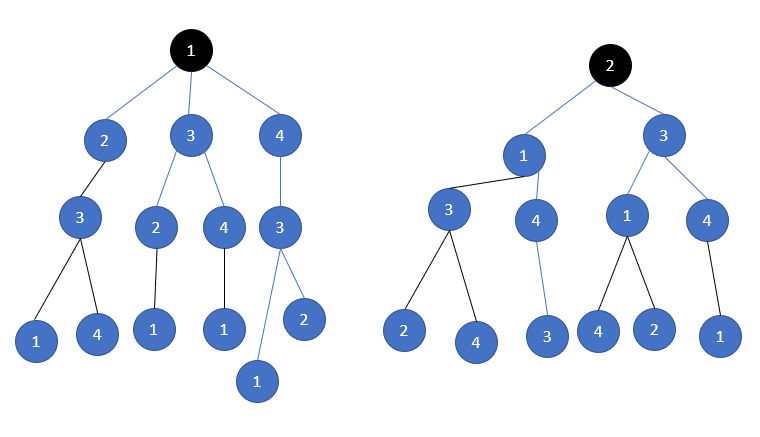
\includegraphics[width=.8\linewidth]{comptree12.png}
			\label{63c1}
			\caption{Unrolled comp trees for snodes 1 2}
		\end{subfigure}%
		\begin{subfigure}{.5\textwidth}
			\centering
			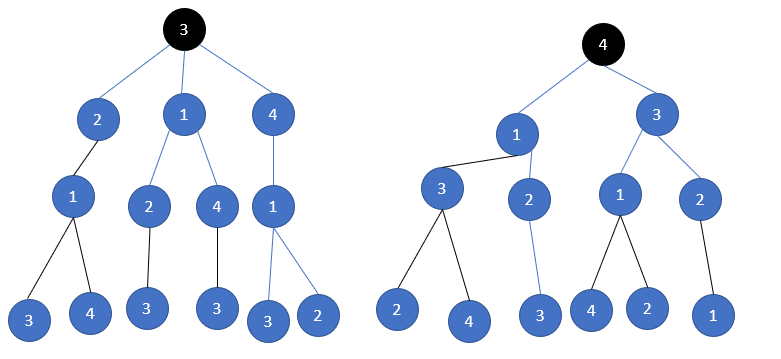
\includegraphics[width=.8\linewidth]{comptree34.png}
			\label{63c2}
			\caption{Unrolled comp trees for snodes 3 4}
		\end{subfigure}
		\label{63c}
		\caption{unrolled to depth 3}
	\end{figure}
The below demonstrates the information matrix for our computation tree starting at node 1 after unrolling 2 of the three levels listed above. Note that r = $\rho$
\begin{verbatim}
	[[1,-r,r,r,0,0,0,0],
	[-r,1,0,0,r,0,0,0],
	[r,0,1,0,0,r,r,0],
	[r,0,0,1,0,0,0,r],
	[0,r,0,0,1,0,0,0],
	[0,0,r,0,0,1,0,0],
	[0,0,r,0,0,0,1,0],
	[0,0,0,r,0,0,0,1]]
\end{verbatim}
As to its positive definiteness, it is in fact positive definite. Again you can see the code used to calculate this in the appendix. This holds for both values 0.39 and 0.40, but appears to break down at 0.5. If we were to continue to expand the tree and test the matrix, we would see that it fails to be positive definite at even earlier values. Due to this, I suspect that it may even become non positive definite at 0.4, which would make sense why our naive approach of belief propagation would not converge.
\end{section}

\begin{section}{Appendix}
	All code can be found here: https://github.com/bogyshi/CSE515/tree/master/HW/hw3
	\\
	code for question 4.6 is in q462.py
	\\
	code for question 5.1 is in q51d.py
	\\
	and code for question 63 is in q63.py
\end{section}
\end{document}

